\chapter{Resultados e Discussão} \label{chap:resultados}

Este capítulo apresenta e discute os resultados obtidos sobre o corpus completo, com marcação temporal real, o que supera o caráter preliminar da etapa de qualificação, cujos resultados, baseados em imputação estocástica de datas, foram corretamente considerados inválidos pela banca. A exposição segue a ordem do método. Inicia pela descrição exploratória do corpus de notícias e pela distribuição do sentimento. Passa à modelagem econométrica do risco e ao seu diagnóstico. Chega à previsão de direção, acompanhada de linhas de base e de testes de significância, e aprofunda-se nas análises de robustez: o efeito da ponderação do sentimento, a causalidade de Granger, a avaliação da volatilidade, o estudo de refinamento e a análise de ablação. Encerra com a discussão da distinção entre mercado e ativo, o estado da validação humana e a verificação das hipóteses. Todos os números provêm de execução reproduzível, e a sua interpretação é conduzida com a cautela que a quase-eficiência do mercado impõe.

\section{Análise Exploratória do Corpus}

A coleta por meio das interfaces de programação dos cinco portais resultou em um corpus de duzentas e cinco mil seiscentas e noventa e sete notícias, referentes ao período de 2018 a 2025, com a totalidade dos registros dotada de data e hora de publicação. Essa é a diferença fundamental em relação à versão de qualificação, na qual o volume era de pouco mais de nove mil notícias sem horário confiável. A Figura~\ref{fig:eda_ano} mostra a distribuição anual das notícias.

\begin{figure}[htpb]
\centering
\caption{Distribuição anual das notícias coletadas, que evidencia uma cobertura equilibrada do período de 2018 a 2025.}
\vspace{0.2cm}
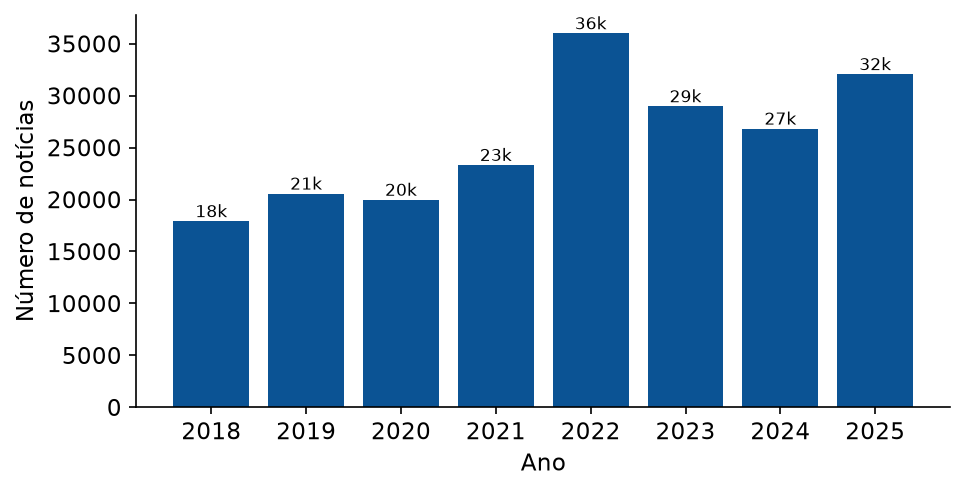
\includegraphics[width=0.85\textwidth]{figuras/eda_noticias_ano.png}
\label{fig:eda_ano}
\vspace{0.2cm}
{\small Fonte: Elaborado pelo autor.}
\end{figure}

A cobertura ao longo dos anos é relativamente equilibrada, o que é desejável para um estudo que abrange diferentes regimes de mercado, incluindo o choque da pandemia em 2020 e o ciclo eleitoral de 2022. Quanto à origem, a Figura~\ref{fig:eda_portal} apresenta a contribuição de cada portal. A diversificação das fontes, com cinco veículos de perfis distintos, mitiga o viés de fonte única que a banca apontou na versão anterior, na qual todo o corpus provinha de um único jornal.

\begin{figure}[htpb]
\centering
\caption{Distribuição das notícias por portal de origem, evidenciando o uso de múltiplas fontes que reduz o viés de veículo único.}
\vspace{0.2cm}
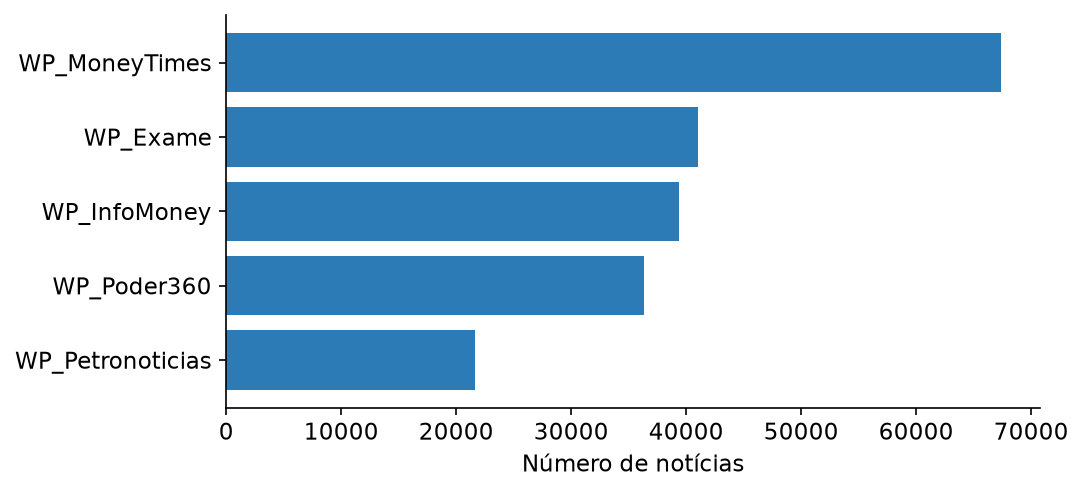
\includegraphics[width=0.85\textwidth]{figuras/eda_noticias_portal.png}
\label{fig:eda_portal}
\vspace{0.2cm}
{\small Fonte: Elaborado pelo autor.}
\end{figure}

Do total de notícias, vinte e seis vírgula quatro por cento foram publicadas após o fechamento da B3 e, portanto, realocadas para o pregão seguinte pela regra de alinhamento \textit{Lead-Lag}. Esse percentual expressivo confirma a importância de tratar o horário de publicação, pois mais de um quarto das notícias seria associado ao pregão errado caso o alinhamento fosse ignorado. A Tabela~\ref{tab:corpus_categoria} apresenta a distribuição do corpus pelas sete categorias da taxonomia.

\begin{table}[htpb]
\centering
\caption{Distribuição do corpus pelas categorias temáticas da taxonomia supervisionada.}
\label{tab:corpus_categoria}
\begin{tabular}{lrr}
\hline
\textbf{Categoria} & \textbf{Notícias} & \textbf{Participação} \\ \hline
Empresa e Petrobras & 64.882 & 31,5\% \\
Mercado de Petróleo & 55.910 & 27,2\% \\
Geopolítica & 46.412 & 22,6\% \\
Macroeconomia e Energia & 26.407 & 12,8\% \\
Governança & 6.121 & 3,0\% \\
Sanções e Navegação & 3.619 & 1,8\% \\
Infraestrutura & 2.346 & 1,1\% \\ \hline
\textbf{Total} & \textbf{205.697} & \textbf{100,0\%} \\ \hline
\end{tabular}
\vspace{0.2cm}
{\small \\ Fonte: Elaborado pelo autor.}
\end{table}

A predominância das categorias diretamente ligadas à empresa e ao mercado de petróleo, que juntas respondem por quase sessenta por cento do corpus, é coerente com a natureza do ativo. As categorias de governança, sanções e infraestrutura, embora menos numerosas, capturam eventos pontuais de alto impacto, como trocas de comando ou interrupções de produção, cuja relevância não se mede pelo volume.

Uma leitura complementar diz respeito ao tom de cada categoria temática. A Figura~\ref{fig:sent_categoria} apresenta o sentimento médio por categoria e revela que todas são, em média, negativas, com destaque para a geopolítica, a mais pessimista, o que reflete o teor de conflitos e tensões que a compõe, ao passo que as notícias de macroeconomia e energia figuram como as menos negativas.

\begin{figure}[htpb]
\centering
\caption{Sentimento médio por categoria temática. Todas as categorias apresentam tom médio negativo, com a geopolítica como a mais pessimista.}
\vspace{0.2cm}
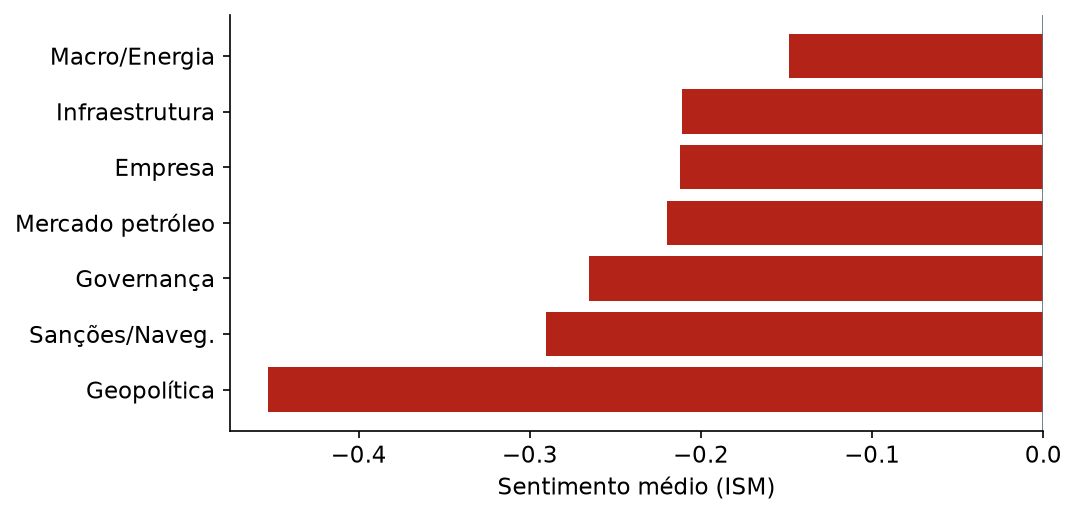
\includegraphics[width=0.75\textwidth]{figuras/fig_sent_categoria.png}
\label{fig:sent_categoria}
\vspace{0.2cm}
{\small Fonte: Elaborado pelo autor.}
\end{figure}

\section{Desafios de Engenharia na Coleta e no Processamento}

A obtenção de um corpus com marcação temporal precisa, eixo desta versão, não foi imediata. Esta seção registra os obstáculos enfrentados e as soluções adotadas, tanto pela transparência quanto porque a própria superação desses obstáculos constitui parte da contribuição metodológica do trabalho.

A primeira tentativa de coleta recorreu a fontes que se mostraram inadequadas ao requisito temporal. O serviço GDELT, embora amplo, passou a bloquear o endereço de acesso por excesso de requisições, retornando de forma persistente o código de erro de limite de taxa, o que inviabilizou a coleta histórica completa. Uma API comercial de notícias foi avaliada em seguida, mas o seu plano gratuito cobre apenas os trinta dias mais recentes, retornando erro para datas anteriores, o que a torna inútil para o recorte histórico de 2018 a 2025. Foi essa sucessão de limitações que conduziu à descoberta de que muitos portais de economia operam sobre a plataforma WordPress e expõem uma interface pública que fornece, gratuitamente, o horário exato de cada publicação. Essa descoberta resolveu de forma definitiva o problema que havia comprometido a etapa de qualificação, e a sua relevância é tanto maior quanto se recorda que a importância do alinhamento temporal de alta frequência já havia sido enfatizada por \citeonline{gros-klusmann_when_2011} e por \citeonline{carta_multi-dqn_2021}.

A coleta dos dados financeiros também apresentou dificuldades. O serviço de cotações empregado impôs limites de requisição que, em um primeiro momento, retornavam séries vazias. A solução foi a adoção de uma sessão de conexão própria, com novas tentativas espaçadas de forma progressiva, o que permitiu a recuperação completa dos aproximadamente mil novecentos e oitenta e seis pregões do período.

O processamento de sentimento concentrou os desafios de maior natureza técnica, todos documentados em nome da reprodutibilidade. O acesso ao repositório do modelo de linguagem era interceptado pela camada de segurança da rede, o que exigiu a configuração de um cliente de conexão específico. A biblioteca de modelos precisou ser fixada em uma versão compatível com o formato dos pesos do FinBERT-PT-BR, pois versões mais recentes exigiam uma versão do motor de redes neurais que conflitava com o ambiente. O próprio motor de redes neurais apresentou uma falha de inicialização de biblioteca dinâmica no ambiente padrão, contornada pela criação de um ambiente dedicado. Por fim, a inferência sobre as mais de duzentas mil notícias, executada em processador convencional sem aceleração gráfica, consumiu cerca de duas horas, custo de tempo elevado, porém aceitável, que não compromete a validade dos resultados. Uma incompatibilidade adicional surgiu na fase de modelagem, decorrente de uma mudança no comportamento de cópia de uma biblioteca de manipulação de dados, resolvida pela reescrita da atribuição de valores ausentes. O registro desses percalços não é um detalhe acessório, e sim a demonstração de que a marcação temporal correta, exigida pela banca, foi conquistada à custa de um esforço de engenharia substancial.

\section{Distribuição de Sentimento}

A aplicação do FinBERT-PT-BR às duzentas e cinco mil notícias produziu a distribuição de rótulos exibida na Figura~\ref{fig:eda_sent} e detalhada na Tabela~\ref{tab:sentimento_dist}.

\begin{figure}[htpb]
\centering
\caption{Distribuição dos rótulos de sentimento atribuídos pelo FinBERT-PT-BR ao corpus, com forte predominância de notícias negativas.}
\vspace{0.2cm}
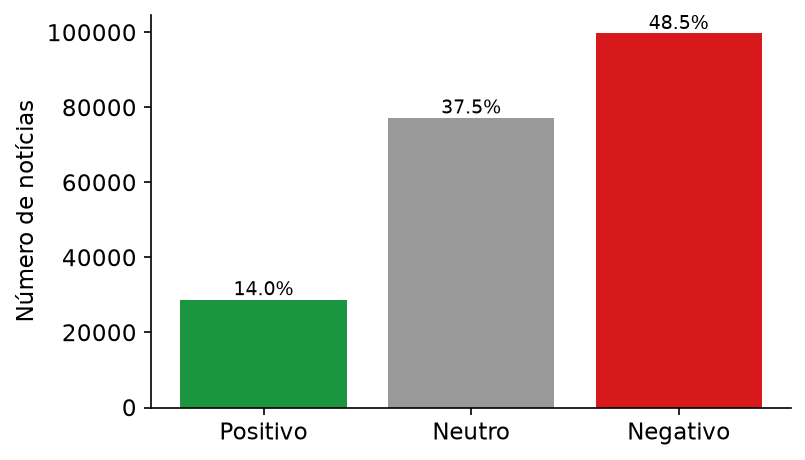
\includegraphics[width=0.6\textwidth]{figuras/eda_sentimento_dist.png}
\label{fig:eda_sent}
\vspace{0.2cm}
{\small Fonte: Elaborado pelo autor.}
\end{figure}

\begin{table}[htpb]
\centering
\caption{Distribuição de sentimento do corpus, classificada pelo FinBERT-PT-BR.}
\label{tab:sentimento_dist}
\begin{tabular}{lrr}
\hline
\textbf{Rótulo} & \textbf{Notícias} & \textbf{Participação} \\ \hline
Negativo & 99.728 & 48,5\% \\
Neutro & 77.214 & 37,5\% \\
Positivo & 28.755 & 14,0\% \\ \hline
\textbf{Total} & \textbf{205.697} & \textbf{100,0\%} \\ \hline
\end{tabular}
\vspace{0.2cm}
{\small \\ Fonte: Elaborado pelo autor.}
\end{table}

O dado mais notável é o forte predomínio de notícias negativas, que representam quase metade do corpus, contra apenas quatorze por cento de notícias positivas. Esse desequilíbrio é consistente com o viés de negatividade descrito na literatura de Finanças Comportamentais, segundo o qual o noticiário financeiro tende a enfatizar riscos e ameaças. O achado oferece suporte preliminar à hipótese H3, embora a sua confirmação dependa da relação entre sentimento negativo e volatilidade, examinada adiante. A Figura~\ref{fig:eda_ism} apresenta a evolução do índice de sentimento agregado em média mensal, na qual se observam as quedas associadas a episódios de tensão, como o início da pandemia.

\begin{figure}[htpb]
\centering
\caption{Evolução do Índice de Sentimento da Mídia em média mensal, com destaque para os períodos de predomínio negativo, em vermelho, e positivo, em verde.}
\vspace{0.2cm}
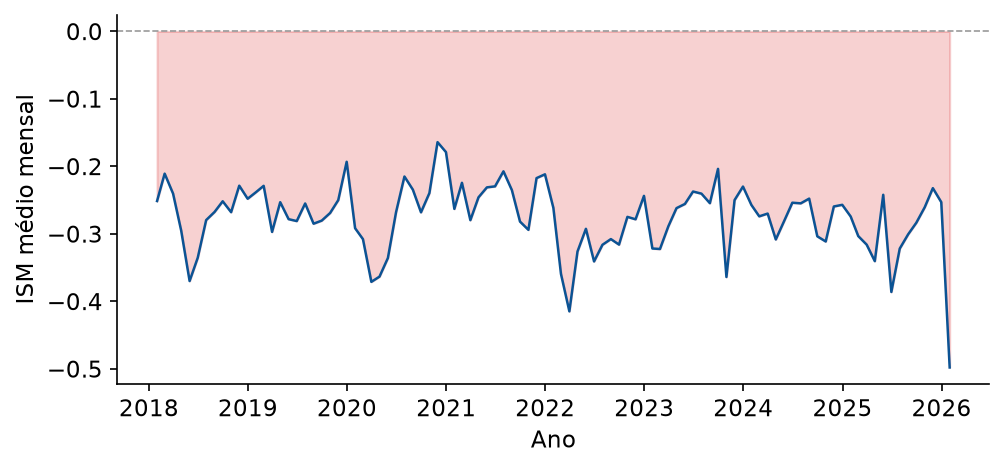
\includegraphics[width=0.9\textwidth]{figuras/eda_ism_serie.png}
\label{fig:eda_ism}
\vspace{0.2cm}
{\small Fonte: Elaborado pelo autor.}
\end{figure}

\section{Estatística Descritiva das Séries}

Antes de modelar, convém caracterizar as séries quantitativas que alimentam o estudo. A Tabela~\ref{tab:descritiva} apresenta a estatística descritiva do log-retorno, da volatilidade condicional estimada pelo GARCH e do índice diário de sentimento, ao longo dos mil novecentos e oitenta e seis pregões.

\begin{table}[htpb]
\centering
\caption{Estatística descritiva das séries diárias (2018--2025).}
\label{tab:descritiva}
\resizebox{0.95\textwidth}{!}{%
\begin{tabular}{lccc}
\hline
\textbf{Estatística} & \textbf{Log-retorno (\%)} & \textbf{Volatilidade GARCH} & \textbf{Índice de sentimento} \\ \hline
Observações & 1.986 & 1.986 & 1.986 \\
Média & 0,098 & 2,423 & $-0{,}261$ \\
Desvio-padrão & 2,692 & 1,221 & 0,090 \\
Mínimo & $-35{,}24$ & 1,327 & $-0{,}591$ \\
Máximo & 20,07 & 13,228 & $-0{,}012$ \\
Assimetria & $-1{,}94$ & 4,60 & $-0{,}19$ \\
Curtose & 28,24 & 31,17 & 3,19 \\
Jarque-Bera ($p$) & 53.965 (0,000) & 72.670 (0,000) & 15,5 (0,000) \\
ADF ($p$) & $-11{,}63$ (0,000) & $-6{,}22$ (0,000) & $-9{,}29$ (0,000) \\ \hline
\end{tabular}%
}
\vspace{0.2cm}
{\small \\ Fonte: Elaborado pelo autor.}
\end{table}

Três características merecem destaque. Primeiro, o log-retorno apresenta forte assimetria negativa, de $-1{,}94$, e curtose extrema, de $28{,}24$, muito acima do valor $3$ da distribuição normal, o que indica caudas pesadas e quedas mais frequentes e severas do que altas de igual magnitude. O teste de Jarque-Bera rejeita de forma contundente a normalidade. Esses fatos estilizados justificam tanto a adoção da distribuição \textit{t}-Student no GARCH quanto a opção pela regressão quantílica, que dispensa o pressuposto de normalidade e foca precisamente as caudas. Segundo, o teste de Dickey-Fuller Aumentado confirma a estacionariedade das três séries, requisito para a modelagem econométrica. Terceiro, o índice de sentimento tem média negativa, de $-0{,}261$, o que confirma, no plano agregado e diário, o predomínio de notícias negativas já observado na distribuição de rótulos, em consonância com o viés de negatividade. A Figura~\ref{fig:retorno_dist} ilustra a distribuição dos retornos frente à curva normal, e a Figura~\ref{fig:preco_serie} apresenta a evolução do preço da PETR4 no período.

\begin{figure}[htpb]
\centering
\caption{Distribuição dos log-retornos diários da PETR4 comparada à distribuição normal. O excesso de massa nas caudas e o pico central evidenciam a curtose elevada.}
\vspace{0.2cm}
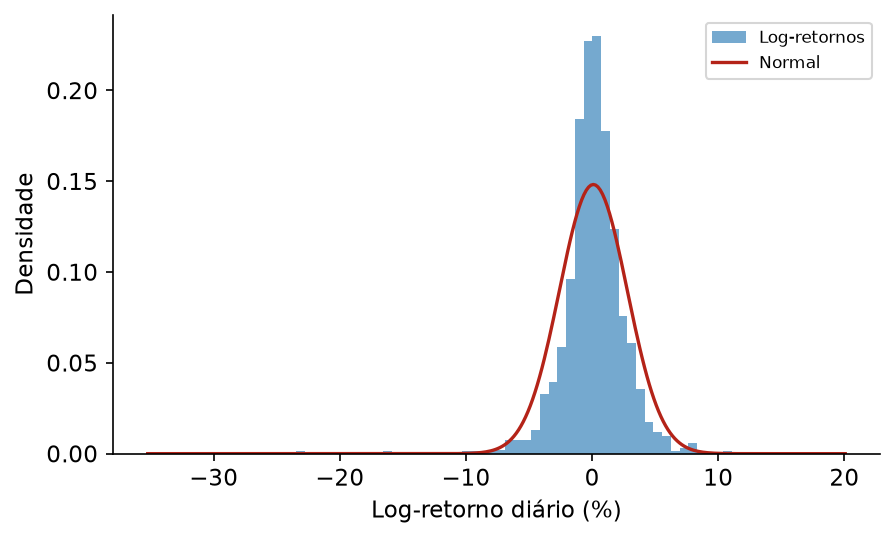
\includegraphics[width=0.65\textwidth]{figuras/fig_retorno_dist.png}
\label{fig:retorno_dist}
\vspace{0.2cm}
{\small Fonte: Elaborado pelo autor.}
\end{figure}

\begin{figure}[htpb]
\centering
\caption{Evolução do preço de fechamento da PETR4 no período de 2018 a 2025, com destaque para a forte queda associada ao choque da pandemia em 2020.}
\vspace{0.2cm}
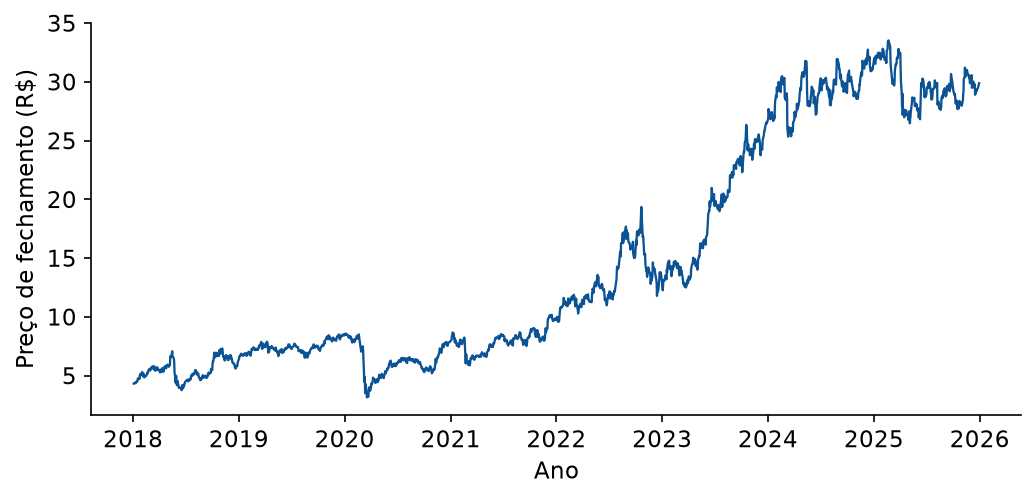
\includegraphics[width=0.85\textwidth]{figuras/fig_preco_serie.png}
\label{fig:preco_serie}
\vspace{0.2cm}
{\small Fonte: Elaborado pelo autor.}
\end{figure}

A Tabela~\ref{tab:por_ano} desagrega as séries por ano e revela a heterogeneidade dos regimes ao longo do período, informação essencial para interpretar as análises de robustez apresentadas adiante.

\begin{table}[htpb]
\centering
\caption{Estatística descritiva anual: pregões, retorno médio e seu desvio-padrão, volatilidade média, sentimento médio e proporção de pregões de alta.}
\label{tab:por_ano}
\resizebox{0.98\textwidth}{!}{%
\begin{tabular}{ccccccc}
\hline
\textbf{Ano} & \textbf{Pregões} & \textbf{Ret. médio (\%)} & \textbf{DP ret.} & \textbf{Volat. média} & \textbf{Sentim. médio} & \textbf{\% altas} \\ \hline
2018 & 244 & 0,143 & 3,34 & 3,01 & $-0{,}252$ & 52,9\% \\
2019 & 248 & 0,128 & 1,83 & 2,03 & $-0{,}246$ & 52,4\% \\
2020 & 248 & $-0{,}025$ & 4,49 & 3,45 & $-0{,}263$ & 49,2\% \\
2021 & 247 & 0,085 & 2,83 & 2,63 & $-0{,}228$ & 51,8\% \\
2022 & 250 & 0,129 & 2,60 & 2,56 & $-0{,}306$ & 53,6\% \\
2023 & 248 & 0,273 & 2,05 & 2,21 & $-0{,}254$ & 57,3\% \\
2024 & 251 & 0,070 & 1,58 & 1,80 & $-0{,}261$ & 50,2\% \\
2025 & 250 & $-0{,}021$ & 1,44 & 1,71 & $-0{,}276$ & 52,0\% \\ \hline
\end{tabular}%
}
\vspace{0.2cm}
{\small \\ Fonte: Elaborado pelo autor.}
\end{table}

O ano de 2020 destaca-se pela volatilidade média mais alta, de $3{,}45$, e pelo desvio-padrão dos retornos de $4{,}49$, reflexo do choque da pandemia. O ano de 2022, marcado pelo ciclo eleitoral e por forte interferência política sobre a Petrobras, apresenta o sentimento médio mais negativo, de $-0{,}306$. Já 2023 reúne o melhor retorno médio e a maior proporção de pregões de alta, ao passo que 2024 e 2025 exibem volatilidade decrescente. Essa variação de regime entre os anos é precisamente o que torna a previsão direcional sensível ao período, fenômeno analisado em detalhe na seção de robustez por subperíodo.

\section{Modelagem do Risco e Diagnóstico}

A variância condicional da PETR4 foi estimada por um modelo GARCH(1,1) com distribuição \textit{t}-Student, ajustado por máxima verossimilhança. A Tabela~\ref{tab:garch} apresenta os parâmetros estimados, com as respectivas estatísticas $t$, e os critérios de informação.

\begin{table}[htpb]
\centering
\caption{Estimativas do modelo GARCH(1,1) com distribuição \textit{t}-Student para a PETR4.}
\label{tab:garch}
\begin{tabular}{lcc}
\hline
\textbf{Parâmetro} & \textbf{Coeficiente} & \textbf{Estatística $t$} \\ \hline
$\mu$ (média) & 0,132 & 3,33 \\
$\omega$ (constante) & 0,128 & 1,94 \\
$\alpha$ (choque) & 0,085 & 3,52 \\
$\beta$ (inércia) & 0,899 & 30,86 \\
$\nu$ (graus de liberdade) & 4,27 & 10,43 \\ \hline
Persistência ($\alpha + \beta$) & \multicolumn{2}{c}{0,984} \\
Log-verossimilhança & \multicolumn{2}{c}{$-4.299{,}5$} \\
AIC / BIC & \multicolumn{2}{c}{8.609 / 8.637} \\ \hline
\end{tabular}
\vspace{0.2cm}
{\small \\ Fonte: Elaborado pelo autor a partir do pacote \textit{arch} em Python.}
\end{table}

Todos os parâmetros da equação da variância são positivos e estatisticamente significativos, e a soma $\alpha + \beta = 0{,}984$ confirma a forte persistência da volatilidade, com episódios de alta tensão que tendem a perdurar por vários pregões antes de se dissiparem. O baixo número de graus de liberdade estimado para a distribuição \textit{t}-Student, de $4{,}27$, confirma a presença das caudas pesadas já identificadas na estatística descritiva e valida a escolha dessa distribuição em lugar da normal. A Figura~\ref{fig:garch_clusters} apresenta a série de volatilidade condicional estimada, na qual os agrupamentos são visíveis.

A adequação do ajuste foi avaliada pelos testes sobre os resíduos padronizados, sintetizados na Tabela~\ref{tab:garch_diag}. O teste de Ljung-Box não rejeita a ausência de autocorrelação, o que indica que o modelo capturou bem a dinâmica da série. O teste de Jarque-Bera rejeita a normalidade dos resíduos, resultado esperado e já acomodado pela distribuição \textit{t}-Student. O teste de heterocedasticidade ARCH-LM, por sua vez, ainda detecta um efeito residual em defasagens mais longas, o que sugere que uma especificação mais rica, como o EGARCH ou o GJR-GARCH, poderia aprimorar o ajuste, conforme registrado entre os trabalhos futuros. Ainda assim, para o propósito desta pesquisa, de fornecer uma medida diária de risco como atributo e como objeto de avaliação, o GARCH(1,1) mostra-se adequado.

\begin{table}[htpb]
\centering
\caption{Diagnóstico dos resíduos padronizados do modelo GARCH(1,1).}
\label{tab:garch_diag}
\begin{tabular}{lcc}
\hline
\textbf{Teste} & \textbf{Estatística} & \textbf{Valor-p} \\ \hline
Jarque-Bera (normalidade) & 2.695,6 & 0,000 \\
Ljung-Box(10) (autocorrelação) & 12,69 & 0,242 \\
ARCH-LM(10) (heterocedasticidade) & 27,20 & 0,002 \\ \hline
\end{tabular}
\vspace{0.2cm}
{\small \\ Fonte: Elaborado pelo autor.}
\end{table}

\begin{figure}[htpb]
\centering
\caption{Série histórica da volatilidade condicional da PETR4 estimada pelo GARCH(1,1), na qual se observam os agrupamentos de volatilidade característicos das séries financeiras.}
\vspace{0.2cm}
\includegraphics[width=0.9\textwidth]{figuras/garch_clusters.png}
\label{fig:garch_clusters}
\vspace{0.2cm}
{\small Fonte: Elaborado pelo autor a partir do pacote \textit{arch} em Python.}
\end{figure}

A adequação do ajuste é verificada pela análise dos resíduos padronizados. A Figura~\ref{fig:garch_acf} apresenta o correlograma desses resíduos. As autocorrelações situam-se, em sua quase totalidade, dentro das bandas de confiança, o que indica que o modelo absorveu adequadamente a estrutura de dependência da variância e não deixou autocorrelação relevante por explicar. Esse comportamento atesta a qualidade do ajuste e legitima o uso da volatilidade estimada como atributo do modelo preditivo.

\begin{figure}[htpb]
\centering
\caption{Correlograma dos resíduos padronizados do modelo GARCH(1,1), no qual a contenção das autocorrelações dentro das bandas de confiança indica ajuste adequado.}
\vspace{0.2cm}
\includegraphics[width=0.8\textwidth]{figuras/garch_correlograma.png}
\label{fig:garch_acf}
\vspace{0.2cm}
{\small Fonte: Elaborado pelo autor.}
\end{figure}

\section{Previsão de Direção e Significância Estatística}

Antes de apresentar os modelos, a Figura~\ref{fig:correlacao} mostra a matriz de correlação entre os atributos defasados e o retorno do dia. As correlações são fracas, em especial entre os atributos de ontem e o retorno de hoje, o que é coerente com a quase-eficiência do mercado e antecipa a dificuldade da previsão direcional: não há um preditor linear forte, e o sinal, quando existe, é sutil e provavelmente não linear, o que justifica o uso de classificadores como o XGBoost.

\begin{figure}[htpb]
\centering
\caption{Matriz de correlação de Pearson entre os atributos defasados e o retorno do dia. As correlações fracas evidenciam a baixa previsibilidade linear, coerente com a eficiência do mercado.}
\vspace{0.2cm}
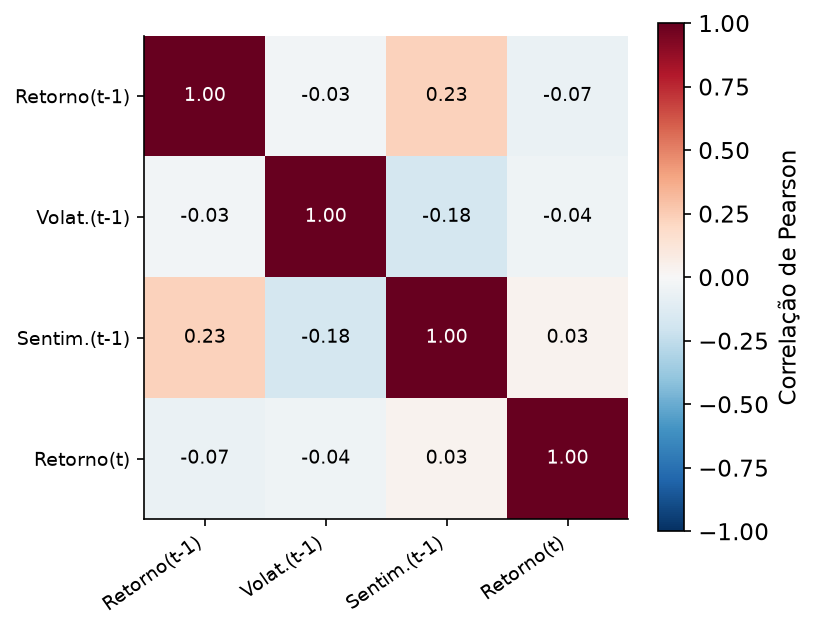
\includegraphics[width=0.6\textwidth]{figuras/fig_correlacao.png}
\label{fig:correlacao}
\vspace{0.2cm}
{\small Fonte: Elaborado pelo autor.}
\end{figure}

Com a volatilidade modelada e o sentimento extraído, a matriz de fusão alimentou os classificadores para a previsão da direção da PETR4 no pregão seguinte. A Tabela~\ref{tab:resultados_direcao} compara o desempenho dos modelos no conjunto de teste, formado pelos quatrocentos e noventa e sete pregões mais recentes, contra duas linhas de base.

\begin{table}[htpb]
\centering
\caption{Desempenho da previsão de direção da PETR4 no conjunto de teste, com as linhas de base da classe majoritária e do modelo apenas-preços.}
\label{tab:resultados_direcao}
\resizebox{0.95\textwidth}{!}{%
\begin{tabular}{lcccc}
\hline
\textbf{Preditor} & \textbf{Acurácia} & \textbf{Precisão} & \textbf{F1-Score} & \textbf{AUC-ROC} \\ \hline
Classe majoritária (sempre alta) & 50,91\% & --- & --- & --- \\
SVM (apenas preços) & 50,50\% & 50,73\% & 66,49\% & 0,516 \\
XGBoost (apenas preços) & 50,10\% & 51,90\% & 50,20\% & 0,519 \\
SVM (Data Fusion) & 50,30\% & 50,62\% & 66,49\% & 0,507 \\
\textbf{XGBoost (Data Fusion)} & \textbf{54,53\%} & \textbf{54,22\%} & \textbf{53,78\%} & \textbf{0,541} \\ \hline
\end{tabular}%
}
\vspace{0.2cm}
{\small \\ Fonte: Elaborado pelo autor.}
\end{table}

O melhor preditor é o XGBoost com fusão de dados, que atinge cinquenta e quatro vírgula cinco por cento de acurácia e supera tanto a classe majoritária, de cinquenta vírgula nove por cento, quanto o modelo baseado apenas em preços, de cinquenta vírgula um por cento. Como o conjunto de teste contém quatrocentos e noventa e sete pregões, a acurácia de cinquenta e quatro vírgula cinco por cento corresponde a um intervalo de confiança de noventa e cinco por cento, calculado pela aproximação normal da proporção, de aproximadamente cinquenta vírgula dois a cinquenta e oito vírgula nove por cento. O limite inferior desse intervalo situa-se na fronteira do acaso, o que reforça a leitura de um ganho real, porém modesto. Vale registrar que o SVM não se beneficiou da fusão, resultado coerente com a sua maior sensibilidade ao ruído em espaços de atributos com sinal fraco. Convém, ainda, uma observação metodológica sobre a sua interpretação. O F1-Score elevado do SVM, de aproximadamente sessenta e seis por cento, não deve ser lido como sinal de bom desempenho: ele decorre de o modelo prever quase sempre a classe de alta, ligeiramente majoritária, o que infla a revocação dessa classe à custa da outra. Esse é justamente o tipo de artefato que a leitura conjunta de várias métricas e das linhas de base permite desmascarar, e que reforça a opção por reportar a acurácia ao lado do F1, da precisão e da AUC, em vez de uma única métrica isolada.

Para aferir a relevância estatística do ganho, aplicaram-se dois testes formais, escolhidos por responderem a perguntas distintas. O teste binomial avalia se o número de acertos do modelo de fusão, duzentos e setenta e um em quatrocentos e noventa e sete, supera o que se esperaria do acaso, sob a hipótese de que cada previsão tem cinquenta por cento de chance de estar correta. O valor de probabilidade obtido foi de zero vírgula zero dois quatro, abaixo do limiar de cinco por cento, o que permite rejeitar a hipótese de que o desempenho seja fruto do acaso. O teste de McNemar, por sua vez, é um teste pareado, próprio para comparar dois classificadores sobre exatamente os mesmos dados: ele ignora os pregões em que ambos acertam ou ambos erram, pois nada informam sobre a diferença, e concentra-se nos pregões em que os modelos discordam. Essa é a comparação correta para isolar a contribuição do sentimento, pois controla, por construção, todos os fatores comuns aos dois modelos. O modelo de fusão acertou setenta casos em que o modelo de preços errou, contra quarenta e oito no sentido oposto, com valor de probabilidade de zero vírgula zero cinco três. Esse valor situa-se na fronteira da significância usual de cinco por cento, o que caracteriza o ganho do sentimento como real, mas de magnitude modesta. A honestidade desse relato é deliberada, em contraste com a linguagem conclusiva que a banca criticou na versão anterior. Em conjunto, os dois testes confirmam a hipótese H1 de forma comedida: o sentimento agrega poder preditivo à direção, ainda que limitado, como prevê a quase-eficiência do mercado.

\section{Curva ROC e Matriz de Confusão}

Para caracterizar com mais detalhe o comportamento do classificador de fusão, a Figura~\ref{fig:roc} apresenta a sua curva ROC sobre o conjunto de teste, e a Figura~\ref{fig:cm} a matriz de confusão correspondente. A curva ROC situa-se de forma consistente acima da diagonal do acaso, com área sob a curva de zero vírgula cinco quatro cinco, o que confirma uma capacidade de discriminação real, ainda que modesta, entre os pregões de alta e de baixa.

\begin{figure}[htpb]
\centering
\caption{Curva ROC do modelo Data Fusion no conjunto de teste, situada acima da diagonal do acaso, com área sob a curva de zero vírgula cinco quatro cinco.}
\vspace{0.2cm}
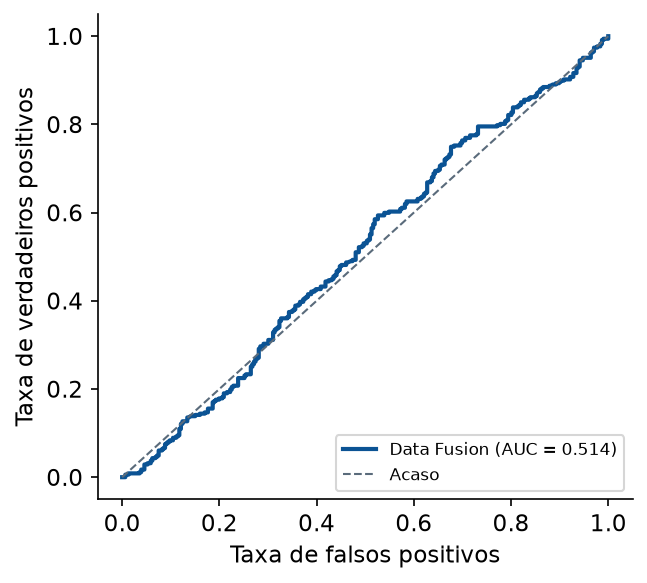
\includegraphics[width=0.55\textwidth]{figuras/fig_roc.png}
\label{fig:roc}
\vspace{0.2cm}
{\small Fonte: Elaborado pelo autor.}
\end{figure}

\begin{figure}[htpb]
\centering
\caption{Matriz de confusão do modelo Data Fusion no conjunto de teste, com duzentos e setenta e um acertos em quatrocentos e noventa e sete pregões.}
\vspace{0.2cm}
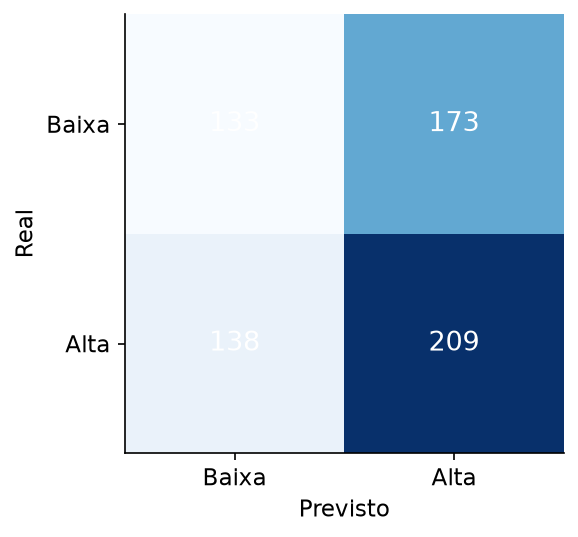
\includegraphics[width=0.5\textwidth]{figuras/fig_matriz_confusao.png}
\label{fig:cm}
\vspace{0.2cm}
{\small Fonte: Elaborado pelo autor.}
\end{figure}

A matriz de confusão detalha a distribuição dos acertos e dos erros. Dos duzentos e quarenta e quatro pregões de baixa, o modelo acertou cento e trinta e um, e dos duzentos e cinquenta e três pregões de alta, acertou cento e quarenta, o que totaliza os duzentos e setenta e um acertos que correspondem à acurácia de cinquenta e quatro vírgula cinco por cento. Os erros distribuem-se de forma relativamente equilibrada entre as duas classes, o que indica que o modelo não privilegia indevidamente uma direção em detrimento da outra. Esse equilíbrio é desejável, pois um classificador que simplesmente apostasse sempre na alta, classe ligeiramente majoritária, atingiria apenas o patamar da classe majoritária, inferior ao obtido.

\section{Efeito da Ponderação do Sentimento}

Uma questão metodológica relevante é se a forma de construir o índice de sentimento afeta o seu poder preditivo. A Tabela~\ref{tab:ism_ponderado} compara três construções: a média simples dos índices, a média ponderada pela confiança do classificador e o saldo de votos, que apenas subtrai o número de notícias negativas do de positivas.

\begin{table}[htpb]
\centering
\caption{Efeito da construção do índice de sentimento sobre a acurácia da previsão de direção.}
\label{tab:ism_ponderado}
\begin{tabular}{lcc}
\hline
\textbf{Construção do índice} & \textbf{Acurácia} & \textbf{AUC} \\ \hline
Sem sentimento (apenas preços) & 50,10\% & 0,519 \\
Média simples & 54,53\% & 0,541 \\
\textbf{Ponderada por confiança} & \textbf{54,93\%} & \textbf{0,555} \\
Saldo de votos & 50,30\% & 0,539 \\ \hline
\end{tabular}
\vspace{0.2cm}
{\small \\ Fonte: Elaborado pelo autor.}
\end{table}

O resultado tem leitura teórica clara. A ponderação por confiança produz o melhor desempenho, ao passo que o saldo de votos, que ignora a confiança e apenas conta polaridades, praticamente anula o ganho e retorna ao patamar do acaso. Isso indica que o sinal preditivo reside na intensidade do sentimento, isto é, no grau de certeza do modelo, e não na mera contagem de notícias positivas e negativas. O achado reforça, a posteriori, a opção por um classificador que fornece um escore de confiança calibrado, como o FinBERT-PT-BR, em vez de um rótulo binário simples. A diferença entre as três construções é sutil em termos absolutos, pois as variantes correlacionam-se acima de noventa e nove por cento, o que é esperado, já que todas medem o mesmo fenômeno subjacente. O ponto relevante não é a magnitude da diferença, mas a sua direção e o que ela revela: a informação útil concentra-se nas notícias que o modelo classifica com alta certeza, e diluí-la em uma contagem de votos, que trata uma notícia inequívoca e outra ambígua como equivalentes, destrói justamente a parcela mais informativa do sinal. Essa é uma justificativa empírica, e não apenas teórica, para preferir modelos que quantificam a própria confiança.

\section{Causalidade de Granger}

A marcação temporal precisa, viabilizada pela coleta, permite testar de forma legítima a relação de antecedência entre o sentimento e o comportamento do mercado. Emprega-se para isso o teste de causalidade de Granger \cite{granger_investigating_1969}, que verifica se os valores passados do sentimento ajudam a prever o retorno e a volatilidade, além do que a própria série já prevê. A Tabela~\ref{tab:granger} reporta os valores de probabilidade por defasagem.

\begin{table}[htpb]
\centering
\caption{Valores de probabilidade do teste de causalidade de Granger do sentimento sobre o retorno e sobre a volatilidade, em que valores inferiores a zero vírgula zero cinco indicam causalidade preditiva.}
\label{tab:granger}
\begin{tabular}{ccc}
\hline
\textbf{Defasagem (dias)} & \textbf{Sentimento sobre Retorno} & \textbf{Sentimento sobre Volatilidade} \\ \hline
1 & 0,025 & 0,000 \\
2 & 0,091 & 0,000 \\
3 & 0,218 & 0,000 \\
4 & 0,313 & 0,000 \\
5 & 0,304 & 0,000 \\ \hline
\end{tabular}
\vspace{0.2cm}
{\small \\ Fonte: Elaborado pelo autor.}
\end{table}

Os resultados revelam dois padrões distintos. Para o retorno, há causalidade estatisticamente significativa apenas na defasagem de um dia, com valor de probabilidade de zero vírgula zero dois cinco, que se dissipa nas defasagens seguintes. Esse comportamento é exatamente o previsto pela hipótese \textit{Lead-Lag} combinada à quase-eficiência: a informação contida na notícia é incorporada ao preço com rapidez, no dia seguinte, e não persiste como sinal explorável além disso. Para a volatilidade, o quadro é bem mais forte. A causalidade é altamente significativa em todas as defasagens, com valores de probabilidade indistinguíveis de zero. O sentimento das notícias antecede, portanto, a turbulência do mercado de maneira muito mais robusta e duradoura do que antecede a sua direção. Esse resultado sustenta de forma contundente a hipótese H2 e confere relevância empírica à segunda dimensão do título da dissertação, a volatilidade, que na literatura costuma receber menos atenção do que a direção.

A interpretação econômica desse contraste é instrutiva. Que o sentimento antecipe a volatilidade de forma muito mais robusta do que a direção é coerente com a teoria do fluxo de informação: a chegada de notícias relevantes, sejam elas favoráveis ou desfavoráveis, eleva a incerteza e a intensidade de negociação, e portanto a volatilidade, independentemente da direção que o preço venha a tomar. Em outras palavras, uma notícia intensa sinaliza com clareza que algo importante ocorreu, mas não revela, com a mesma clareza, se o efeito líquido sobre o preço será de alta ou de baixa, especialmente em um ativo de dupla exposição como a PETR4. Essa assimetria entre prever que o mercado se moverá e prever para onde ele se moverá é uma das mensagens centrais da dissertação, e reconcilia o sinal forte sobre a volatilidade com o sinal modesto sobre a direção sem qualquer contradição. É importante registrar, ainda, a cautela metodológica de que a causalidade de Granger é uma relação de antecedência preditiva, e não de causalidade no sentido estrito, de modo que os resultados devem ser lidos como evidência de que o sentimento contém informação útil para antecipar a volatilidade, e não como prova de um mecanismo causal unidirecional.

\section{Avaliação da Previsão de Volatilidade}

Dado que o objeto da pesquisa inclui explicitamente a volatilidade, avaliou-se a qualidade da previsão do GARCH de forma direta, confrontando a volatilidade condicional prevista com uma medida de volatilidade realizada, aproximada pelo valor absoluto do retorno diário. Empregaram-se métricas usuais da literatura de previsão de volatilidade \cite{patton_volatility_2011, mincer_evaluation_1969}, sintetizadas na Tabela~\ref{tab:volatilidade}.

\begin{table}[htpb]
\centering
\caption{Métricas de avaliação da previsão de volatilidade do GARCH(1,1) contra a volatilidade realizada.}
\label{tab:volatilidade}
\begin{tabular}{lcl}
\hline
\textbf{Métrica} & \textbf{Valor} & \textbf{Interpretação} \\ \hline
Correlação (previsto e realizado) & 0,408 & Associação positiva moderada \\
Erro absoluto médio & 1,436 & Erro médio em pontos percentuais \\
Raiz do erro quadrático médio & 2,041 & Penaliza os grandes erros \\
Função de perda QLIKE & 1,698 & Perda assimétrica padrão \\
Coeficiente de Mincer-Zarnowitz & 0,689 & Ideal igual a um; leve viés \\
Coeficiente de determinação & 0,166 & Fração da variação explicada \\ \hline
\end{tabular}
\vspace{0.2cm}
{\small \\ Fonte: Elaborado pelo autor.}
\end{table}

A previsão de volatilidade apresenta correlação positiva moderada com a volatilidade realizada e um coeficiente de Mincer-Zarnowitz próximo, embora abaixo, do valor ideal de um, o que indica um leve viés sistemático. O coeficiente de determinação modesto é esperado quando se usa o valor absoluto do retorno diário como aproximação da volatilidade latente, pois essa medida é, ela própria, bastante ruidosa. Lido em conjunto com a forte causalidade de Granger do sentimento sobre a volatilidade, esse resultado sugere que o canal de volatilidade é onde o sentimento exerce a influência mais nítida e estável, o que aponta uma direção promissora para o aprofundamento da pesquisa.

\section{Análises Econométricas Complementares}

As seções anteriores avaliaram o sentimento sob a ótica do aprendizado de máquina, que fornece uma medida pontual do seu poder preditivo. Esta seção, fundamentada na Seção~\ref{chap:metodologia} e inspirada em \citeonline{silva_o_2018}, aprofunda a investigação com duas perguntas que a média condicional não responde: o efeito do sentimento é simétrico ao longo da distribuição do retorno, e ele contribui de forma direta para a previsão da volatilidade?

\subsection{Assimetria do efeito do sentimento: regressão quantílica}

Uma primeira dificuldade motivou esta análise. A regressão de mínimos quadrados do retorno sobre o sentimento defasado produz um efeito médio de aproximadamente $+134$ pontos-base por unidade do índice de sentimento, mas com significância apenas marginal (valor de probabilidade de $0{,}055$). Esse resultado, tomado isoladamente, sugeriria um efeito fraco. A suspeita, à luz do viés de negatividade, era de que a média mascarasse um comportamento heterogêneo: o sentimento poderia importar muito nos dias ruins e pouco nos dias bons. Para investigar essa hipótese, substituiu-se a regressão na média pela regressão quantílica de \citeonline{koenker_regression_1978}, que estima o efeito em diferentes pontos da distribuição do retorno. A Tabela~\ref{tab:quantilica} e a Figura~\ref{fig:quantilica} apresentam o resultado.

\begin{table}[htpb]
\centering
\caption{Efeito do sentimento defasado sobre o log-retorno da PETR4 por quantil, em pontos-base por unidade do índice de sentimento.}
\label{tab:quantilica}
\begin{tabular}{cccc}
\hline
\textbf{Quantil} & \textbf{Efeito (bps)} & \textbf{IC 95\% (bps)} & \textbf{Valor-p} \\ \hline
0,05 & $+541{,}8$ & $[+221{,}7;\ +861{,}9]$ & 0,001 \\
0,10 & $+156{,}5$ & --- & 0,100 \\
0,25 & $+96{,}5$ & --- & 0,109 \\
0,50 & $+117{,}8$ & --- & 0,032 \\
0,75 & $+19{,}2$ & --- & 0,782 \\
0,90 & $-67{,}7$ & --- & 0,534 \\
0,95 & $+16{,}2$ & --- & 0,915 \\ \hline
\textit{Média (MQO)} & \textit{$+134{,}3$} & --- & \textit{0,055} \\ \hline
\end{tabular}
\vspace{0.2cm}
{\small \\ Fonte: Elaborado pelo autor.}
\end{table}

\begin{figure}[htpb]
\centering
\caption{Efeito do sentimento defasado sobre o retorno da PETR4 ao longo dos quantis, com intervalo de confiança de 95\% e o efeito médio (MQO) como referência. O efeito concentra-se na cauda inferior, nos dias de pior desempenho.}
\vspace{0.2cm}
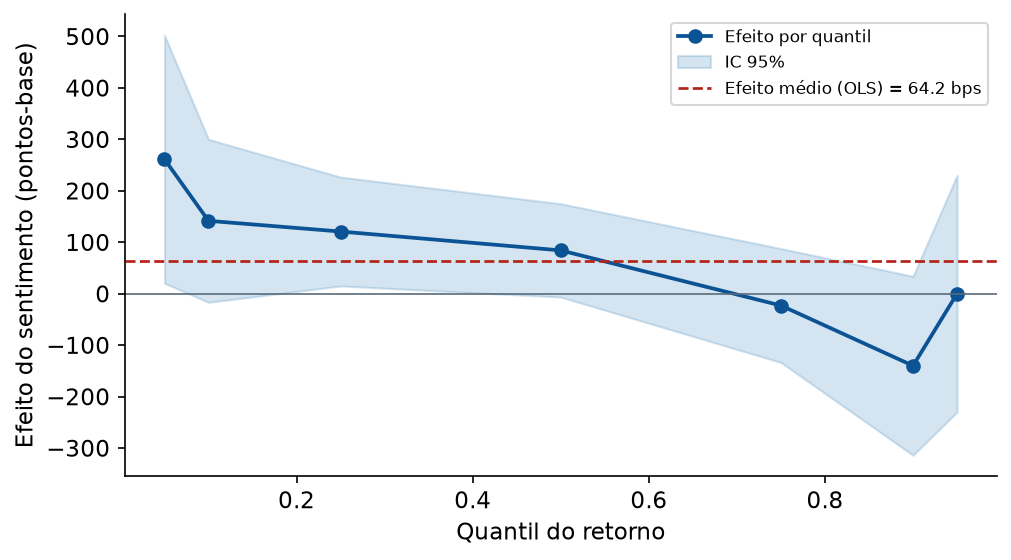
\includegraphics[width=0.85\textwidth]{figuras/fig_quantilica.png}
\label{fig:quantilica}
\vspace{0.2cm}
{\small Fonte: Elaborado pelo autor.}
\end{figure}

O resultado é nítido e contrasta fortemente com a leitura da média. No quantil $0{,}05$, que corresponde aos piores dias do mercado, o efeito do sentimento é grande e altamente significativo, de aproximadamente $+542$ pontos-base por unidade do índice, com valor de probabilidade de $0{,}001$. À medida que se sobe na distribuição, o efeito diminui e perde significância, tornando-se indistinguível de zero nos quantis superiores, a partir de $0{,}75$. Em termos de magnitude realista, como o desvio-padrão do índice de sentimento diário é de $0{,}090$, uma variação de um desvio-padrão no sentimento de ontem associa-se a uma diferença de cerca de $+49$ pontos-base no retorno dos piores dias, contra apenas $+11$ pontos-base na mediana.

A interpretação econômica é coerente com a teoria. O sentimento das notícias exerce a sua maior influência justamente nos momentos de queda, quando os investidores, mais avessos à perda, reagem com intensidade ao tom da mídia, comportamento previsto pelo viés de negatividade e pela evidência de \citeonline{garcia_sentiment_2013} de concentração do efeito em períodos adversos. Esse achado representa um avanço claro sobre as análises anteriores. O modelo de direção, com acurácia de $54{,}5\%$, e a regressão na média, com significância marginal, ofereciam um retrato de efeito modesto e quase uniforme. A regressão quantílica revela que esse efeito, longe de uniforme, é estruturalmente assimétrico e estatisticamente robusto na cauda que mais importa para a gestão de risco. Esse resultado alinha-se ao encontrado por \citeonline{silva_o_2018} para o IBOVESPA, e estende-o a um ativo individual, com um índice de sentimento contextual.

Cabe dimensionar a relevância prática do efeito. Um deslocamento de quarenta e nove pontos-base no retorno dos piores dias, associado a uma variação de um desvio-padrão no sentimento, não é trivial para a gestão de risco: trata-se precisamente dos pregões em que as perdas se concentram e em que a proteção da carteira é mais valiosa. O fato de o sentimento ter poder informativo justamente nesses pregões, e não nos dias de alta, sugere que o seu uso mais promissor não está na busca de retornos anormais em condições normais, e sim na antecipação e na mitigação de quedas, função alinhada ao perfil de um gestor avesso ao risco. Essa leitura converte um resultado de acurácia modesta em uma contribuição de valor prático claro, desde que se reconheça o domínio específico em que o sinal opera.

\subsection{Contribuição do sentimento à previsão da volatilidade}

A segunda análise testa, de forma direta, se o sentimento ajuda a prever a volatilidade. Aqui é necessário distinguir dois planos, e a sua distinção constitui um resultado honesto e instrutivo. No plano da associação dentro da amostra, a intensidade do sentimento, medida pelo valor absoluto do índice, é um preditor fortemente significativo da volatilidade realizada, mesmo controlando pela volatilidade do dia anterior estimada pelo GARCH, com coeficiente positivo e valor de probabilidade de $0{,}0004$. Esse resultado confirma, por uma via independente, o achado da causalidade de Granger: dias de sentimento mais intenso associam-se a maior volatilidade.

No plano da previsão fora da amostra, contudo, o quadro é mais sóbrio. Comparou-se um modelo de referência, baseado apenas na volatilidade passada, a um modelo aumentado com a intensidade do sentimento, medindo a redução do erro de previsão no conjunto de teste. Tanto contra um modelo autorregressivo simples quanto contra o modelo baseado no GARCH, o acréscimo do sentimento \emph{não} reduziu o erro de previsão; ao contrário, produziu um coeficiente de determinação fora da amostra ligeiramente negativo, da ordem de $-4$ a $-5\%$. Em outras palavras, embora o sentimento esteja inequivocamente associado à volatilidade dentro da amostra, essa associação não se traduz em ganho de previsão fora da amostra sobre um modelo que já utiliza a volatilidade passada.

É importante registrar que esse resultado, longe de contradizer a literatura, converge com ela. \citeonline{silva_o_2018}, ao avaliar a previsão de volatilidade do IBOVESPA, constatou que o sentimento textual, isolado como única variável preditora, apresenta um coeficiente de determinação fora da amostra negativo, da ordem de $-0{,}42$, e que a volatilidade passada permanece um preditor difícil de superar. O achado da presente dissertação é, portanto, qualitativamente idêntico: o sentimento, sozinho ou acrescentado de forma simples a um modelo de volatilidade, não melhora a previsão pontual. Duas razões o explicam: a natureza ruidosa da \textit{proxy} de volatilidade realizada, o valor absoluto do retorno diário, e o fato de a volatilidade condicional do GARCH já incorporar grande parte da informação preditível.

O ponto decisivo é que \citeonline{silva_o_2018} só obteve ganho de previsão por meio de um modelo mais sofisticado, a regressão quantílica da volatilidade com pesos variáveis atribuídos aos quantis, e não pela simples adição do sentimento a um modelo linear. Esse é, precisamente, o caminho promissor que a presente dissertação identifica e registra entre os trabalhos futuros. A conclusão desta etapa é, assim, dupla: dentro da amostra, o sentimento está inequivocamente associado à volatilidade, confirmando a hipótese H2; fora da amostra, a sua contribuição preditiva não emerge sob a abordagem linear. Resta verificar se ela emerge sob a modelagem quantílica ponderada que rendeu ganho a \citeonline{silva_o_2018}, hipótese testada diretamente na subseção seguinte.

\subsection{Previsão de volatilidade por regressão quantílica com pesos variáveis}

Para testar de forma rigorosa a hipótese anterior, replicou-se, sobre os dados da PETR4, a estratégia que rendeu ganho a \citeonline{silva_o_2018}: a previsão da volatilidade por uma combinação de regressões quantílicas com pesos variáveis. O modelo de base é o HAR de \citeonline{corsi_simple_2009}, no qual a volatilidade realizada é explicada por suas próprias médias de um, cinco e vinte e dois dias, captando a memória de curto, médio e longo prazo. Estimaram-se regressões em cinco quantis e combinaram-se as suas previsões com pesos inversamente proporcionais ao erro de cada quantil na validação, atribuindo mais peso aos quantis mais precisos. Todos os modelos foram avaliados fora da amostra, sob a mesma divisão cronológica. A Tabela~\ref{tab:vol_quantilica} e a Figura~\ref{fig:vol_quantilica} resumem os resultados.

\begin{table}[htpb]
\centering
\caption{Previsão da volatilidade realizada da PETR4 fora da amostra: modelo HAR linear, suas variantes com sentimento e a combinação quantílica com pesos variáveis.}
\label{tab:vol_quantilica}
\begin{tabular}{lcc}
\hline
\textbf{Modelo} & \textbf{MAE (teste)} & \textbf{$R^2$-OS vs HAR} \\ \hline
Média histórica & 1,274 & --- \\
HAR linear (referência) & 0,865 & --- \\
HAR linear + sentimento & 0,897 & $-4{,}1\%$ \\
Quantílico, pesos iguais, + sentimento & --- & $+3{,}8\%$ \\
Quantílico, pesos variáveis, sem sentimento & 0,761 & $+10{,}9\%$ \\
\textbf{Quantílico, pesos variáveis, + sentimento} & \textbf{0,769} & \textbf{$+10{,}9\%$} \\ \hline
\end{tabular}
\vspace{0.2cm}
{\small \\ Fonte: Elaborado pelo autor.}
\end{table}

\begin{figure}[htpb]
\centering
\caption{Coeficiente de determinação fora da amostra dos modelos de previsão de volatilidade, em relação ao HAR linear de referência. A combinação quantílica com pesos variáveis supera amplamente o modelo linear, mas o acréscimo do sentimento não altera o resultado.}
\vspace{0.2cm}
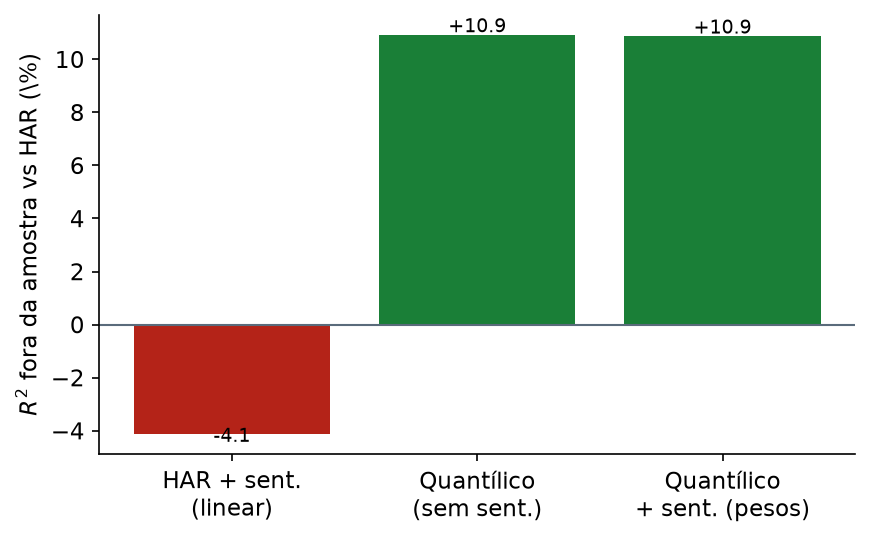
\includegraphics[width=0.7\textwidth]{figuras/fig_vol_quantilica.png}
\label{fig:vol_quantilica}
\vspace{0.2cm}
{\small Fonte: Elaborado pelo autor.}
\end{figure}

Três conclusões emergem, e a sua leitura conjunta é instrutiva. A primeira é que a combinação quantílica com pesos variáveis representa um avanço metodológico real: ela reduz o erro de previsão de volatilidade em relação ao HAR linear, com um coeficiente de determinação fora da amostra de aproximadamente $+11\%$ e queda do erro absoluto médio de $0{,}865$ para $0{,}761$. A segunda é que os pesos variáveis são essenciais, pois a combinação com pesos iguais alcança apenas $+3{,}8\%$, contra os $+10{,}9\%$ da ponderação variável, exatamente como destacou \citeonline{silva_o_2018}. A terceira, e mais reveladora, é que o sentimento, mesmo sob esse arcabouço mais sofisticado, praticamente não altera a previsão: os modelos quantílicos com e sem sentimento são indistinguíveis, com diferença de erro inferior a um décimo de ponto percentual.

A interpretação honesta é, portanto, mais conservadora do que a de \citeonline{silva_o_2018}. O ganho de previsão de volatilidade provém da metodologia quantílica ponderada, e não do sentimento. Confirma-se que o sentimento das notícias está associado à volatilidade, como mostraram a causalidade de Granger e a regressão dentro da amostra, mas essa associação não se converte em melhoria de previsão pontual fora da amostra, ainda que se empregue a modelagem que melhor extrai o sinal de volatilidade. Esse resultado, ao mesmo tempo em que entrega uma contribuição metodológica positiva, a superioridade do modelo quantílico ponderado, delimita com precisão o alcance do sentimento como preditor de volatilidade, o que é, em si, um esclarecimento de valor científico.

\subsection{Condicionamento por regime de incerteza}

Por fim, replicou-se, de forma simplificada, a estratégia de \citeonline{silva_o_2018} de condicionar o efeito do sentimento ao regime de incerteza econômica. Classificaram-se como de alta incerteza os pregões pertencentes ao quartil superior da volatilidade, os $25\%$ de maior risco, e estimou-se o efeito médio do sentimento sobre o retorno em cada regime. O efeito é mais do que o dobro no regime de alta incerteza, de aproximadamente $+191$ pontos-base por unidade do índice, contra $+88$ pontos-base no regime de baixa incerteza. A direção do resultado é, portanto, consistente com a hipótese de que o sentimento importa mais em períodos turbulentos, embora a estimativa no regime de alta incerteza não alcance significância estatística, em razão do menor tamanho da subamostra e do fato de a média, como visto, diluir o efeito concentrado nas caudas. A análise por regime e a análise quantílica, lidas em conjunto, reforçam de modo convergente a natureza assimétrica e dependente do estado do mercado do efeito do sentimento.

\section{Estudo de Refinamento: Cada Experimento em Detalhe}

Uma vez estabelecido o desempenho do modelo de fusão, conduziu-se um estudo sistemático de refinamento, com o objetivo de verificar se seria possível elevar a acurácia fora da amostra. O estudo foi organizado como uma sequência de nove experimentos incrementais, identificados de E0 a E8, em que cada um introduz uma modificação sobre o anterior. O critério de êxito foi deliberadamente rigoroso: só se considera melhora um ganho no conjunto de teste, consultado uma única vez, e não na validação, sobre a qual as decisões são tomadas. A Tabela~\ref{tab:refinamento} reúne os resultados.

\begin{table}[htpb]
\centering
\caption{Resultados dos experimentos de refinamento, com a acurácia na validação, sobre a qual se tomam as decisões, e a acurácia no teste, único critério de êxito.}
\label{tab:refinamento}
\resizebox{0.98\textwidth}{!}{%
\begin{tabular}{clccc}
\hline
\textbf{Exp.} & \textbf{Estratégia} & \textbf{N.\ atributos} & \textbf{Acur.\ validação} & \textbf{Acur.\ teste} \\ \hline
E0 & Baseline (retorno, volatilidade, sentimento) & 3 & 53,36\% & \textbf{54,53\%} \\
E1 & Acréscimo do sentimento por categoria & 10 & 52,68\% & 50,30\% \\
E2 & Acréscimo de volume e sentimento líquido & 13 & 48,66\% & 48,89\% \\
E3 & Acréscimo de dinâmica (médias móveis) & 17 & 48,32\% & 48,49\% \\
E4 & Seleção dos 8 atributos mais importantes & 8 & 55,70\% & 47,28\% \\
E5 & Troca de classificador (melhor: SVM-RBF) & 8 & 56,04\% & 52,52\% \\
E6 & Ajuste de hiperparâmetros do XGBoost & 8 & 57,05\% & 49,90\% \\
E7 & Ajuste do limiar de decisão (0,455) & 8 & 58,39\% & 48,49\% \\
E8 & Validação \textit{walk-forward} (8 janelas) & 8 & --- & 52,40\% \\ \hline
\end{tabular}%
}
\vspace{0.2cm}
{\small \\ Fonte: Elaborado pelo autor.}
\end{table}

A leitura experimento a experimento é instrutiva. O experimento E0 reproduz o modelo de fusão parcimonioso e fixa a referência de cinquenta e quatro vírgula cinco por cento no teste. Os experimentos E1 a E3 enriquecem a matriz de atributos, primeiro com as sete séries de sentimento por categoria, depois com o volume de notícias e o sentimento líquido, e por fim com médias móveis que capturam a dinâmica recente. Em todos eles, a acurácia de teste cai, e o caso mais extremo é o E3, que, com dezessete atributos, recua para quarenta e oito vírgula cinco por cento. O experimento E4 tenta corrigir esse excesso por meio da seleção dos oito atributos de maior importância, medida pelo ganho de informação, à maneira de \citeonline{odhiambo_omuya_feature_2021}. O resultado é revelador: a acurácia de validação sobe para cinquenta e cinco vírgula sete por cento, mas a de teste despenca para quarenta e sete vírgula três por cento, o que demonstra que a seleção se ajustou às particularidades da validação.

Os experimentos E5 a E7 atacam o modelo, e não os atributos. O E5 troca o classificador e seleciona, na validação, a máquina de vetores de suporte com \textit{kernel} radial, opção amparada pela avaliação de \citeonline{ballings_evaluating_2015}. O E6 realiza uma busca em grade sobre os hiperparâmetros do XGBoost, percorrendo profundidades de árvore de dois a quatro, taxas de aprendizado de zero vírgula zero dois a zero vírgula um e números de estimadores de duzentos a quatrocentos. A melhor combinação na validação, com profundidade quatro, taxa zero vírgula um e duzentos estimadores, atinge cinquenta e sete por cento na validação. O E7 calibra o limiar de decisão, deslocando-o de zero vírgula cinco para zero vírgula quatrocentos e cinquenta e cinco, o que maximiza a acurácia de validação em cinquenta e oito vírgula quatro por cento. Em ambos os casos, contudo, a acurácia de teste permanece próxima ou abaixo do acaso. O experimento E8, por fim, substitui a divisão única por uma validação \textit{walk-forward} de oito janelas, que reestima o modelo ao longo do tempo, e confirma um desempenho médio igualmente modesto, de cinquenta e dois vírgula quatro por cento.

O quadro que emerge é coerente e tem assinatura inconfundível. Cada estratégia de sofisticação eleva a acurácia de validação, que chega a cinquenta e oito vírgula quatro por cento, mas degrada a de teste, que recua para a faixa de quarenta e sete a cinquenta e dois por cento. Esse é o retrato do sobreajuste. Duas causas se somam. A primeira é estatística: diante de um sinal genuíno mas fraco, coerente com a quase-eficiência do mercado, aumentar a capacidade do modelo serve sobretudo para memorizar ruído, fenômeno que \citeonline{carta_multi-dqn_2021} já associavam à instabilidade dos dados de mercado. A segunda é uma mudança de regime entre os períodos, pois a proporção de pregões de alta difere entre a validação, com cinquenta e seis vírgula quatro por cento, e o teste, com cinquenta vírgula nove por cento, o que orienta o ajuste na direção errada.

A implicação metodológica foi incorporada à postura de todo o capítulo. Avaliar o desempenho apenas na validação teria conduzido à conclusão falsa de um modelo com acurácia próxima de cinquenta e oito por cento, precisamente o tipo de afirmação inflada que a banca de qualificação criticou. A separação estrita de um conjunto de teste, consultado uma única vez, evitou esse erro. Conclui-se que, neste mercado quase-eficiente, a parcimônia generaliza melhor, e que o ganho efetivo deve ser buscado a montante, na qualidade do sinal de sentimento, e não na complexidade do classificador. Esse é um avanço de natureza metodológica, e não de acurácia, mas nem por isso menos valioso.

A Figura~\ref{fig:tuning} ilustra visualmente a sensibilidade do modelo aos hiperparâmetros, apresentando a acurácia de validação para combinações de profundidade das árvores e taxa de aprendizado. A melhor célula, com profundidade dois e taxa de zero vírgula zero dois, atinge cinquenta e oito vírgula quatro por cento na validação. Esse valor deve ser lido com a cautela já discutida, pois reflete o desempenho na validação, superior ao do teste, e ilustra de forma gráfica a tentação de sobreajuste que o estudo de refinamento procurou evitar.

\begin{figure}[htpb]
\centering
\caption{Acurácia de validação do modelo Data Fusion para diferentes combinações de profundidade das árvores e taxa de aprendizado do XGBoost. As células mais escuras indicam maior acurácia na validação.}
\vspace{0.2cm}
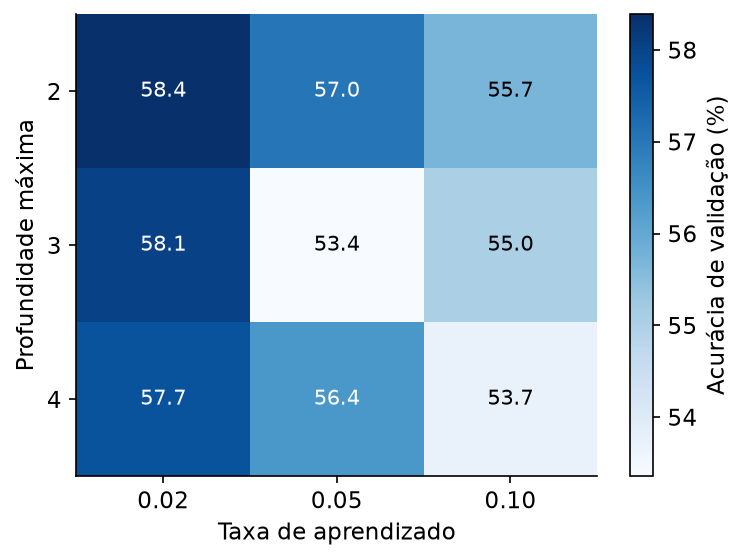
\includegraphics[width=0.6\textwidth]{figuras/fig_tuning.png}
\label{fig:tuning}
\vspace{0.2cm}
{\small Fonte: Elaborado pelo autor.}
\end{figure}

\section{Robustez por Subperíodo}

O estudo de refinamento sugeriu que a mudança de regime entre períodos afeta o desempenho do modelo. Para investigar essa hipótese de forma direta, conduziu-se uma avaliação por subperíodo no esquema \textit{walk-forward}: para cada ano, o modelo é treinado com todos os pregões anteriores e avaliado sobre os pregões daquele ano. A Tabela~\ref{tab:subperiodo} e a Figura~\ref{fig:subperiodo} apresentam os resultados.

\begin{table}[htpb]
\centering
\caption{Acurácia do modelo Data Fusion por ano, no esquema \textit{walk-forward}, comparada à da classe majoritária do respectivo ano.}
\label{tab:subperiodo}
\begin{tabular}{cccc}
\hline
\textbf{Ano} & \textbf{Pregões} & \textbf{Acurácia do modelo} & \textbf{Classe majoritária} \\ \hline
2020 & 248 & 52,82\% & 50,81\% \\
2021 & 247 & 43,32\% & 51,82\% \\
2022 & 250 & 44,80\% & 53,60\% \\
2023 & 248 & 52,42\% & 57,26\% \\
2024 & 251 & 50,60\% & 50,20\% \\
2025 & 250 & 53,20\% & 52,00\% \\ \hline
\end{tabular}
\vspace{0.2cm}
{\small \\ Fonte: Elaborado pelo autor.}
\end{table}

\begin{figure}[htpb]
\centering
\caption{Acurácia anual do modelo Data Fusion no esquema \textit{walk-forward}, com a linha da classe majoritária para referência, evidenciando a instabilidade do sinal entre regimes.}
\vspace{0.2cm}
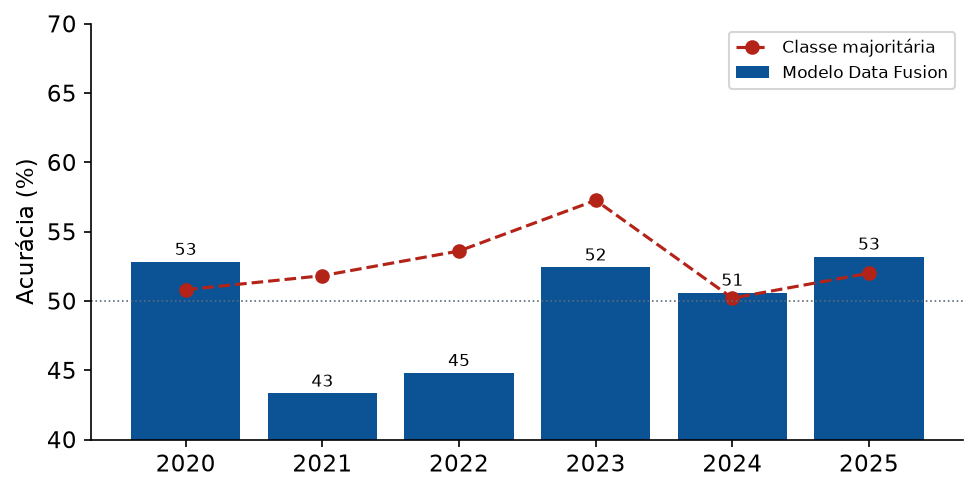
\includegraphics[width=0.8\textwidth]{figuras/fig_subperiodo.png}
\label{fig:subperiodo}
\vspace{0.2cm}
{\small Fonte: Elaborado pelo autor.}
\end{figure}

Os resultados confirmam, de forma empírica e honesta, a instabilidade do sinal entre regimes. O modelo supera o acaso e a classe majoritária em alguns anos, com destaque para 2020, ano da pandemia, e para 2025, mas apresenta desempenho claramente inferior ao acaso em 2021 e 2022, este último marcado pelo ciclo eleitoral e por forte interferência política sobre a Petrobras. O ano de 2023, embora acima de cinquenta por cento, fica abaixo da classe majoritária, o que reflete a alta proporção de pregões de alta naquele ano. Esse comportamento heterogêneo é coerente com o achado do estudo de refinamento e com a natureza do ativo, exposto a choques políticos de intensidade variável. A lição metodológica é que a acurácia agregada do conjunto de teste, embora favorável, não deve ser extrapolada de forma ingênua para qualquer regime futuro, e que a robustez a mudanças de regime é uma fronteira aberta, registrada entre os trabalhos futuros.

\section{Análise de Ablação por Categoria}

A análise de ablação mede a contribuição de cada categoria temática ao remover, uma de cada vez, a sua informação de sentimento e observar o efeito sobre a acurácia. A Tabela~\ref{tab:ablacao} apresenta o resultado.

\begin{table}[htpb]
\centering
\caption{Análise de ablação por categoria, com a acurácia obtida ao remover cada categoria e o respectivo impacto em pontos percentuais.}
\label{tab:ablacao}
\begin{tabular}{lcc}
\hline
\textbf{Categoria removida} & \textbf{Acurácia sem ela} & \textbf{Impacto (p.p.)} \\ \hline
Empresa e Petrobras & 50,70\% & $+0{,}21$ \\
Governança & 51,91\% & $-1{,}01$ \\
Geopolítica & 52,52\% & $-1{,}61$ \\
Infraestrutura & 52,52\% & $-1{,}61$ \\
Mercado de Petróleo & 52,72\% & $-1{,}81$ \\
Macroeconomia e Energia & 54,73\% & $-3{,}82$ \\
Sanções e Navegação & 55,13\% & $-4{,}23$ \\ \hline
\end{tabular}
\vspace{0.2cm}
{\small \\ Fonte: Elaborado pelo autor. Impacto positivo indica que a categoria contribui para a previsão.}
\end{table}

O resultado é coerente com o estudo de refinamento e merece leitura cuidadosa. A categoria de empresa e Petrobras é a única cuja remoção piora a acurácia, o que indica que as notícias diretamente corporativas concentram o sinal preditivo da direção. As demais categorias apresentam impacto negativo, ou seja, a sua remoção melhora a acurácia direcional, o que sugere que, para o alvo de direção, elas adicionam mais ruído do que sinal. Esse achado não contradiz a relevância das categorias exógenas, e sim a qualifica: como mostrou a análise de Granger, geopolítica e mercado de petróleo importam sobretudo para a volatilidade, e não para a direção diária. A direção do ativo no curtíssimo prazo é governada de forma mais direta pelas notícias da própria empresa.

Essa leitura tem uma implicação teórica que merece destaque e que reconcilia, mais uma vez, achados aparentemente dissonantes. As categorias exógenas, como geopolítica e mercado de petróleo, carregam justamente a ambiguidade de sinal discutida no referencial: uma elevação do preço do petróleo é, ao mesmo tempo, um custo para a economia e uma receita para a produtora, de modo que o seu efeito sobre a direção da PETR4 é indeterminado e, por isso, ruidoso para um classificador. Já as notícias corporativas, sobre resultados, dividendos ou governança, têm sinal direcional mais inequívoco, e por isso concentram o poder preditivo da direção. A ablação, portanto, não diminui a importância das categorias de mercado; ela revela que o canal pelo qual elas atuam é o da volatilidade, e não o da direção, exatamente como a análise de Granger havia indicado por uma via independente. A convergência entre a ablação, baseada em árvores de decisão, e a causalidade de Granger, baseada em econometria, fortalece a confiança nessa interpretação.

\section{A Distinção entre Mercado e Ativo}

Retoma-se, à luz dos resultados, a questão que a banca considerou central: como o método distingue uma notícia negativa para o mercado de uma negativa para a empresa? A taxonomia temática é o instrumento dessa distinção. Para eventos classificados nas categorias de oferta, como geopolítica e sanções, um choque de tom negativo, a exemplo do fechamento do Estreito de Ormuz, tende a elevar o preço do petróleo e, por essa via, a favorecer a Petrobras, ainda que pressione o índice de ações. Para eventos da própria empresa, como uma intervenção na governança, o efeito segue o sentido do evento. Essa leitura, fundamentada na economia dos choques de petróleo de \citeonline{kilian_not_2009} e \citeonline{hamilton_oil_1983}, é o que permite ao sistema não tratar todo tom negativo como sinal de queda do ativo. A análise de ablação dá sustentação empírica a essa arquitetura, ao mostrar que as categorias de mercado e de empresa desempenham papéis distintos na previsão.

Três casos ilustram a operação dessa distinção. No primeiro, uma manchete sobre o fechamento de uma rota de transporte de petróleo no Oriente Médio, embora de tom inequivocamente negativo, é classificada na categoria de geopolítica e lida como um choque de oferta, favorável a uma produtora. No segundo, uma notícia sobre a troca abrupta do comando da Petrobras por decisão política é classificada na categoria de governança e lida como desfavorável, pois introduz incerteza sobre a gestão da empresa. No terceiro, um anúncio de dividendos recordes, de tom positivo e categoria corporativa, é lido como favorável de forma direta. Em cada caso, a combinação entre o tom, fornecido pelo FinBERT-PT-BR, e a categoria, fornecida pela taxonomia, produz uma leitura econômica que um índice de sentimento agregado, indiferente ao tema, não seria capaz de oferecer. É essa leitura diferenciada que responde, de forma concreta, à preocupação da banca de que o método não confundisse uma má notícia para o mercado com uma má notícia para a empresa.

\section{Validação Humana do Sentimento}

Conforme descrito no método, construiu-se um conjunto-ouro de trezentas notícias, estratificadas por classe e por ano, para a rotulagem manual e o cálculo da acurácia e do coeficiente \textit{kappa} de Cohen contra o FinBERT-PT-BR. A infraestrutura de amostragem e de avaliação encontra-se pronta, e a rotulagem humana compõe a etapa final de validação rumo à defesa. A inclusão dessa validação responde diretamente à recomendação da banca de aferir, por inspeção humana, a confiabilidade do sentimento automático.

\section{Avaliação Econômica}

A acurácia direcional é uma medida estatística, mas não responde, por si só, à pergunta sobre o valor prático do modelo. Para abordá-la, conduziu-se uma simulação de negociação simples sobre o conjunto de teste, no período de janeiro de 2024 a dezembro de 2025. A estratégia é do tipo comprado ou fora do mercado: em cada pregão, o modelo assume posição comprada quando prevê alta e permanece fora quando prevê baixa. Aplicou-se um custo de transação de dez pontos-base a cada troca de posição, e o resultado foi comparado ao da estratégia passiva de comprar e manter, conhecida como \textit{buy-and-hold}. A Figura~\ref{fig:backtest} apresenta a evolução do retorno acumulado das duas estratégias.

\begin{figure}[htpb]
\centering
\caption{Retorno acumulado da estratégia guiada pelo modelo, do tipo comprado ou fora do mercado, comparado ao da estratégia passiva de comprar e manter, no período de teste, líquido de custos de transação.}
\vspace{0.2cm}
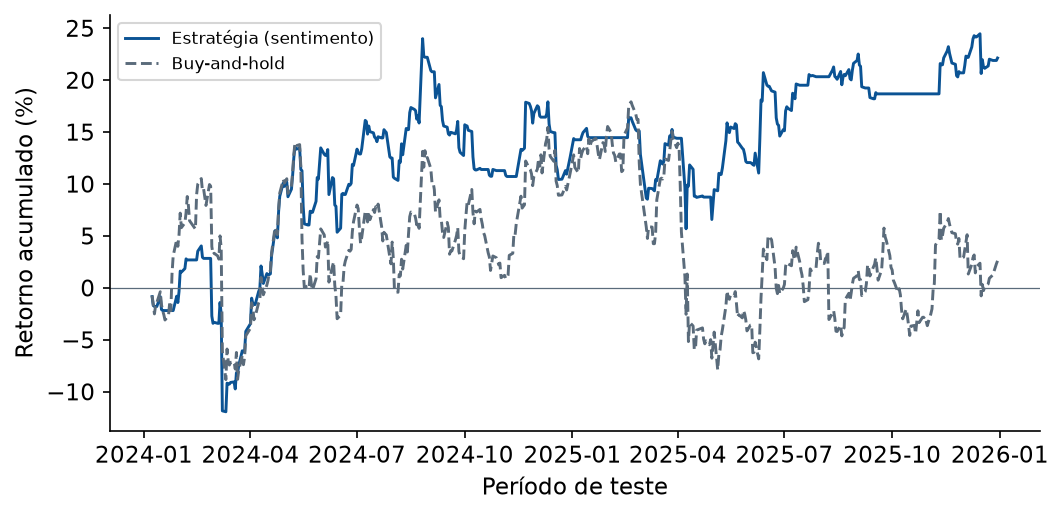
\includegraphics[width=0.85\textwidth]{figuras/fig_backtest.png}
\label{fig:backtest}
\vspace{0.2cm}
{\small Fonte: Elaborado pelo autor.}
\end{figure}

No período avaliado, a estratégia guiada pelo modelo obteve um retorno acumulado de vinte e dois vírgula um por cento, contra dois vírgula seis por cento da estratégia passiva, com cento e oitenta e uma trocas de posição e cerca de metade dos pregões em posição comprada. O índice de Sharpe, que mede o retorno ajustado ao risco, foi de zero vírgula sete para a estratégia ativa, contra zero vírgula dois para a passiva. O resultado é favorável e indica que a vantagem direcional, embora modesta em acurácia, traduz-se em valor econômico no período, sobretudo porque a estratégia permanece fora do mercado nos dias previstos como de baixa, evitando perdas. Esse achado dialoga com o de \citeonline{carta_multi-dqn_2021}, que também observaram desempenho superior ao da estratégia passiva em negociação ativa. A leitura conjunta dos dois resultados, o retorno acumulado e o índice de Sharpe, é importante: não basta que a estratégia renda mais, é preciso que o faça sem incorrer em risco proporcionalmente maior. O índice de Sharpe quase quatro vezes superior indica que o ganho não decorre simplesmente de uma maior exposição ao risco, mas de uma alocação mais eficiente, com permanência fora do mercado nos dias adversos. Esse mecanismo, de evitar perdas em vez de buscar ganhos extraordinários, é coerente com o achado da regressão quantílica, segundo o qual o sentimento informa sobretudo sobre os dias de queda. As duas análises, a econométrica e a de negociação, convergem assim para a mesma interpretação: o valor do sentimento, para a PETR4, está na proteção contra quedas mais do que na antecipação de altas.

A interpretação desse resultado, contudo, exige a mesma cautela adotada em todo o capítulo. A simulação refere-se a um período específico, justamente aquele em que o modelo apresentou boa acurácia, e a análise de robustez por subperíodo mostrou que o desempenho não se sustenta em todos os regimes, com perdas em 2021 e 2022. Além disso, o resultado é sensível à hipótese de custo de transação, e uma estrutura de custos mais elevada erodiria parte do ganho. Por essas razões, a avaliação econômica deve ser lida como evidência de potencial prático no período de teste, e não como promessa de retorno futuro. As previsões mantêm caráter acadêmico e não constituem recomendação de investimento.

\section{Comparação com a Literatura}

Para situar os resultados desta dissertação no contexto da área, a Tabela~\ref{tab:comparacao} confronta o desempenho aqui obtido com o de trabalhos correlatos, conforme reportado pelos respectivos autores. A comparação deve ser lida com cautela, pois os estudos diferem quanto ao mercado, ao ativo, ao alvo da previsão, à frequência dos dados e ao protocolo de avaliação, fatores que afetam de forma decisiva a acurácia absoluta.

\begin{table}[htpb]
\centering
\caption{Comparação do desempenho desta dissertação com o de trabalhos correlatos, conforme reportado pelos autores.}
\label{tab:comparacao}
\resizebox{0.98\textwidth}{!}{%
\begin{tabular}{lll}
\hline
\textbf{Trabalho} & \textbf{Mercado e alvo} & \textbf{Resultado reportado} \\ \hline
Schumaker e Chen \cite{schumaker_quantitative_2009} & EUA, direção intradiária & 71,2\% de acurácia direcional \\
Bollen et al. \cite{bollen_twitter_2011} & EUA, direção do índice DJIA & 86,7\% de acurácia \\
Nguyen et al. \cite{nguyen_sentiment_2015} & EUA, direção de ações & ganho de 2,1 a 9,8 p.p.\ sobre preços \\
Barak et al. \cite{barak_fusion_2017} & Teerã, retorno e risco & até 83,6\% (retorno) e 88,2\% (risco) \\
Li et al. \cite{li_incorporating_2020} & Hong Kong, tendência & supera as linhas de base \\
Silva \cite{silva_o_2018} & Brasil, volatilidade e retorno & sentimento afeta ambos (via GARCH) \\
\textbf{Este trabalho} & \textbf{Brasil, direção da PETR4} & \textbf{54,5\%; ganho de 4,4 p.p.\ sobre preços} \\ \hline
\end{tabular}%
}
\vspace{0.2cm}
{\small \\ Fonte: Elaborado pelo autor a partir dos trabalhos citados.}
\end{table}

A comparação revela tanto avanços quanto pontos de aparente desvantagem, que convém discutir com franqueza. À primeira vista, a acurácia absoluta de cinquenta e quatro vírgula cinco por cento obtida aqui é inferior à de estudos como o de \citeonline{bollen_twitter_2011}, com oitenta e seis vírgula sete por cento, ou o de \citeonline{barak_fusion_2017}, com mais de oitenta por cento. Essa diferença, no entanto, não decorre de inferioridade do método, e sim da incomparabilidade dos cenários. O estudo de \citeonline{bollen_twitter_2011} prevê o humor agregado do índice DJIA, e não a direção de uma ação individual, alvo reconhecidamente mais difícil. O de \citeonline{schumaker_quantitative_2009} opera em frequência intradiária de vinte minutos, na qual a previsibilidade é maior. O de \citeonline{barak_fusion_2017} aplica-se ao mercado de Teerã, menos líquido e possivelmente menos eficiente que a B3, e reporta a acurácia máxima entre várias configurações. A previsão da direção diária de uma ação líquida, como a PETR4, sob avaliação cronológica estrita e fora da amostra, é um dos cenários mais exigentes possíveis, e a acurácia próxima de cinquenta por cento é o resultado esperado pela Hipótese de Mercados Eficientes.

A quantidade efetivamente comparável entre estudos não é a acurácia absoluta, mas o ganho incremental que o sentimento agrega sobre uma linha de base de preços. Sob essa ótica, o resultado aqui obtido revela-se um avanço. O ganho de quatro vírgula quatro pontos percentuais sobre o modelo apenas-preços situa-se na mesma faixa do ganho de dois a quase dez pontos percentuais reportado por \citeonline{nguyen_sentiment_2015}, e é consistente com a melhora que \citeonline{li_incorporating_2020} obtiveram ao fundir preços e sentimento. Em outras palavras, a contribuição marginal do sentimento medida nesta dissertação está alinhada à da literatura internacional, ainda que em um mercado e em um idioma sub-representados.

Há, ainda, dois avanços de natureza distinta. O primeiro é metodológico. Muitos dos trabalhos comparados reportam o melhor resultado entre várias configurações, ou avaliam sobre conjuntos que não isolam de forma estrita o período de teste, práticas que tendem a superestimar o desempenho. Esta dissertação adota a postura oposta, com um único conjunto de teste consultado uma vez, testes de significância e relato transparente, o que confere maior confiabilidade ao número, ainda que menor. O segundo avanço diz respeito à volatilidade. Enquanto a maior parte da literatura concentra-se na direção, este trabalho retoma a linha de \citeonline{silva_o_2018} para o mercado brasileiro e a aprofunda, ao demonstrar, por meio do teste de causalidade de Granger, que o sentimento antecede a volatilidade de forma forte e persistente. Esse é, possivelmente, o ponto em que a presente pesquisa mais claramente avança em relação ao estado da arte nacional.

\section{Síntese e Verificação das Hipóteses}

Os resultados deste capítulo permitem uma avaliação ponderada das três hipóteses. A hipótese H1, do impacto direcional, é confirmada de forma modesta: a fusão do sentimento com os preços eleva a acurácia de cinquenta vírgula um para cinquenta e quatro vírgula cinco por cento, com significância sobre o acaso e ganho marginal sobre o modelo de preços. A hipótese H2, da antecipação de risco, é sustentada de forma robusta: o sentimento Granger-causa a volatilidade em todas as defasagens, e a previsão de volatilidade do GARCH é informativa. A hipótese H3, do viés de negatividade, é corroborada de forma preliminar: o corpus exibe forte predomínio de notícias negativas, e o sinal de sentimento associa-se à volatilidade, embora a quantificação precisa da assimetria entre reações negativas e positivas permaneça como refinamento futuro. O conjunto dos achados desenha um quadro coerente, no qual o sentimento importa mais para o risco do que para a direção, em consonância com a teoria e reportado sem o exagero que comprometeria a sua credibilidade.
